\documentclass[11pt,a4paper]{article}

\usepackage[utf8]{inputenc}
\usepackage[T1]{fontenc}
\usepackage[spanish, es-nodecimaldot]{babel}
\addto\captionsspanish{\renewcommand{\tablename}{Tabla}}
\usepackage{geometry}
\geometry{margin=2.5cm}
\usepackage{booktabs}
\usepackage{array}
\usepackage{multirow}
\usepackage{longtable}
\usepackage{hyperref}
\hypersetup{colorlinks=true, linkcolor=black, urlcolor=blue}
\usepackage{parskip}
\usepackage{listings}
\usepackage{xcolor}
\usepackage{enumitem}
\usepackage{graphicx}
\usepackage{url}
\graphicspath{{diagrams/}}
\usepackage{float}
\usepackage{caption}
\usepackage{rotating}
\usepackage{pdflscape}
\usepackage{colortbl}
\usepackage{amssymb}
\usepackage{inconsolata}

\definecolor{pblue}{rgb}{0.13,0.13,1}
\definecolor{pgreen}{rgb}{0,0.5,0}
\definecolor{pred}{rgb}{0.9,0,0}
\definecolor{pgrey}{rgb}{0.46,0.45,0.48}
\definecolor{lightgray}{gray}{0.92}
\definecolor{codered}{RGB}{180,30,30}
\definecolor{codegreen}{RGB}{0,120,0}
\definecolor{codegray}{RGB}{100,100,100}
\definecolor{warnorange}{RGB}{200,100,0}

\lstset{
  language=Java,
  basicstyle=\ttfamily\footnotesize,
  keywordstyle=\color{pblue},
  commentstyle=\color{codegray}\itshape,
  stringstyle=\color{pred},
  showstringspaces=false,
  showspaces=false,
  showtabs=false,
  breaklines=true,
  breakatwhitespace=false,
  postbreak=\mbox{\textcolor{codegray}{$\hookrightarrow$}\space},
  frame=single,
  framesep=4pt,
  xleftmargin=6pt,
  xrightmargin=6pt,
  aboveskip=6pt,
  belowskip=6pt,
  numbers=left,
  numberstyle=\tiny\color{codegray},
  numbersep=5pt,
  captionpos=b
}
\renewcommand{\lstlistingname}{Listado}

\newcommand{\code}[1]{\texttt{#1}}
\newcommand{\bad}[1]{\textcolor{codered}{\textbf{#1}}}
\newcommand{\good}[1]{\textcolor{codegreen}{\textbf{#1}}}
\newcommand{\warn}[1]{\textcolor{warnorange}{\textbf{#1}}}
\setlength{\emergencystretch}{3em}

\title{Análisis de impacto cruzado y opciones de rediseño\\
       \large Paquete \code{org.openmarkov.core.model.network.potential}\\[4pt]
       \normalsize Continuación del análisis previo \emph{rediseño-potenciales}}
\author{Manuel Arias Calleja}
\date{Mayo de 2026}

\begin{document}
\maketitle
\tableofcontents
\newpage

\section*{Resumen ejecutivo}

Este documento extiende el análisis previo del paquete \code{potential}
(\emph{rediseño-potenciales}, marzo de 2026) con un \textbf{mapa exhaustivo del
acoplamiento externo}: qué módulos usan qué clases, métodos y campos del
paquete, y dónde rompería cada decisión de refactor. El recuento principal:

\begin{itemize}[leftmargin=*]
  \item \textbf{372} ficheros \code{.java} importan algo del paquete; \textbf{317}
        referencian alguna variante de \code{TablePotential}.
  \item \textbf{0} subclases externas de cualquier subtipo de \code{Potential}.
        Toda la jerarquía de potenciales vive dentro del paquete.
  \item \textbf{14} \code{@PotentialPanelPlugin} en \code{org.openmarkov.gui}
        que mencionan clases concretas de potencial por literal de clase.
  \item \textbf{315} accesos externos a \code{getValues()[i]} (lectura), de los
        cuales \textbf{7} son escrituras directas en producción.
  \item \textbf{63} invocaciones externas a métodos mutadores específicos de
        potenciales (\code{setValues}, \code{setUncertainValues},
        \code{setNoisyParameters}, \code{setLeakyParameters}, \code{setBranches},
        \code{setRootVariable}\dots).
  \item Cadena \code{instanceof} de \textbf{14 subtipos} en
        \code{PGMXWriter\_0\_2.java:746--860}: punto único que hay que tocar para
        cada nuevo potencial.
\end{itemize}

A la luz de estos datos, la recomendación se confirma: las opciones de
\emph{Nivel~1} (higiene local) y \emph{Nivel~2} (consolidación de capacidades)
son seguras y rentables; las de \emph{Nivel~3} (composición y/o inmutabilidad
estricta) están condicionadas por puntos concretos de mutación y por el
contrato de los plugins GUI/PGMX. El plan de acción se estructura en cinco
fases incrementales (\ref{sec:plan}), cada una con criterios de aceptación y
riesgo evaluado contra los datos de impacto de la sección~\ref{sec:impacto}.

\section{Contexto y alcance}

\subsection{Documento previo y diferencias con éste}

En \code{org.openmarkov/docs/rediseno-potenciales/} ya existe un análisis de
diseño del paquete (marzo de 2026), centrado en problemas \emph{intra}-paquete
(triple responsabilidad de \code{TablePotential}, jerarquía paralela
\code{Strategic\-Table\-Potential}/\code{Uncertain\-Table\-Potential}, abuso de
\code{PotentialRole}, etc.). Ese trabajo culminó con la extracción de las
interfaces de capacidad (\code{Projectable}, \code{Reorderable}, \code{Scalable},
\code{StrategyCarrier}, \code{UncertaintyCarrier}, \code{CEUtilityPotential}) y
la separación parcial de \code{Strategic\-Table\-Potential} y
\code{Uncertain\-Table\-Potential}.

Este documento responde a la pregunta complementaria: \textbf{¿qué impacto
tiene cada paso adicional de rediseño en el resto del workspace?} Por tanto:

\begin{itemize}[leftmargin=*]
  \item No vuelve a discutir los problemas internos ya catalogados; los
        \emph{asume}.
  \item Cataloga el acoplamiento externo con datos cuantitativos
        (\code{file:line}) recogidos sobre el árbol vivo en
        \code{/home/manuel/workspace-openmarkov/}.
  \item Reformula las opciones de refactor en función de su huella en módulos
        externos.
  \item Propone un plan de acción por fases con criterios verificables.
\end{itemize}

\subsection{Inventario rápido del paquete}

Recordatorio breve, sin entrar en detalle (ver el documento previo):

\begin{itemize}[leftmargin=*]
  \item \textbf{Base abstracta:} \code{Potential} (735~líneas) y
        \code{AbstractIndexedPotential}.
  \item \textbf{Interfaces de capacidad:} \code{Projectable},
        \code{Reorderable}, \code{Scalable}, \code{StrategyCarrier},
        \code{UncertaintyCarrier}, \code{CEUtilityPotential}.
  \item \textbf{Tabla densa:} \code{TablePotential} (759~líneas),
        \code{Uncertain\-Table\-Potential}, \code{StrategicTablePotential},
        \code{AugmentedProbTable} y \code{GTable\-Potential<E>}.
  \item \textbf{Definiciones simbólicas:} \code{UniformPotential},
        \code{DeltaPotential}, \code{FunctionPotential},
        \code{LinearCombinationPotential}, \code{GLMPotential},
        \code{ProductPotential}, \code{SumPotential}, \code{SameAsPrevious},
        \code{CycleLengthShift}, \code{ExactDistrPotential}, etc.
  \item \textbf{Distribuciones paramétricas:} \code{BinomialPotential},
        \code{ConditionalGaussianPotential},
        \code{ExponentialPotential},
        \code{ExponentialHazardPotential},
        \code{WeibullHazardPotential},
        \code{DiscretizedCauchyPotential},
        \code{Univariate\-Distr\-Potential}.
  \item \textbf{Subpaquetes:} \code{canonical/} (ICI: Max, Min, Tuning,
        MinMax), \code{treeadd/} (TreeADD\-Potential, TreeADDBranch,
        Threshold), \code{sdag/} (SDAGStrategyTree), \code{plugin/}
        (\code{@PotentialType}, \code{PotentialUtils}).
  \item \textbf{Subpaquete} \code{operation/}: \textasciitilde 4\,169~líneas
        en 15 ficheros. Fachadas (\code{PotentialOperations},
        \code{DiscretePotentialOperations}), implementación interna
        (\code{TablePotentialArithmetic}, \code{*Elimination},
        \code{*Maximization}, \code{*Merge}, \code{*Transform}), descomposiciones
        de utilidad (\code{Marginalization}, \code{SumOutVariable},
        \code{MaxOutVariable}) y auxiliares.
\end{itemize}

\subsection{Jerarquía actual}

La figura~\ref{fig:jerarquia-actual} resume la jerarquía tras el primer
rediseño. Las interfaces de capacidad (azul) ya existen pero su adopción es
parcial: la base \code{Potential} sigue ofreciendo \emph{defaults} para
\code{tableProject}, \code{reorder} y \code{scalePotential} que lanzan
\code{UnsupportedOperationException}.

\begin{figure}[H]
  \centering
  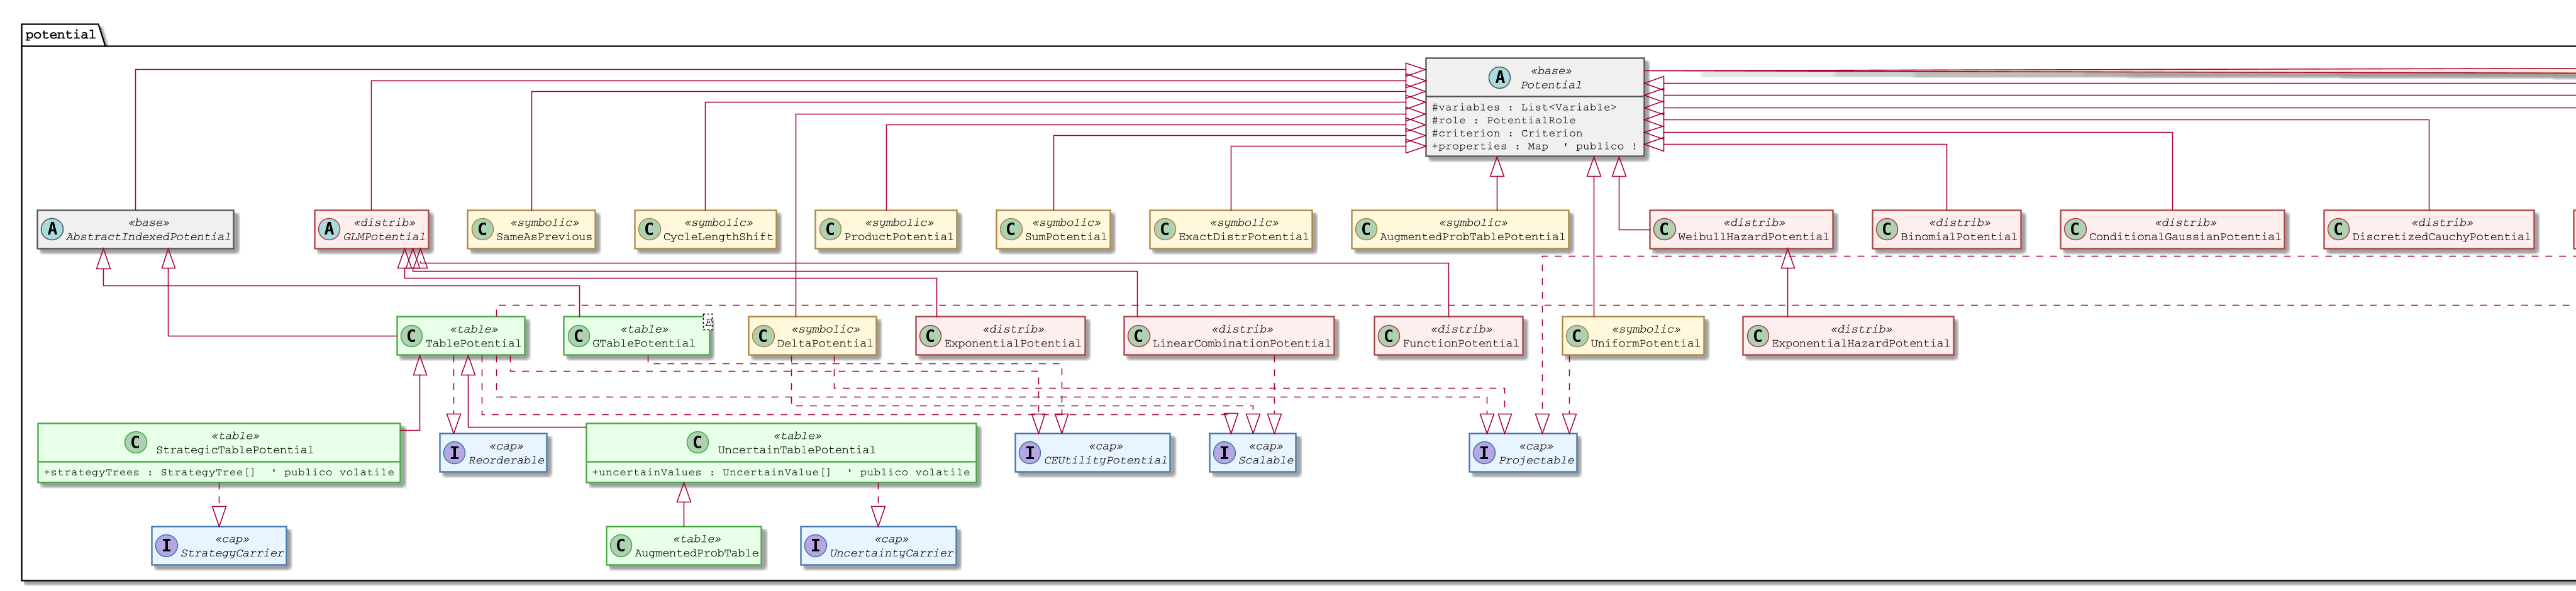
\includegraphics[width=\textwidth]{jerarquia-actual.png}
  \caption{Jerarquía actual del paquete \code{potential} (post Rediseño 1).
           En verde, los \emph{table-potentials}; en amarillo, los simbólicos;
           en rojo claro, las distribuciones paramétricas; en azul, las
           interfaces de capacidad.}
  \label{fig:jerarquia-actual}
\end{figure}

\section{Metodología del análisis cruzado}

Los datos cuantitativos provienen de búsquedas en el árbol
\code{/home/manuel/workspace-openmarkov/} con las exclusiones siguientes:

\begin{itemize}[leftmargin=*]
  \item Se excluye \code{target/}, \code{build/}, \code{out/} y cualquier
        artefacto generado.
  \item Se excluye el propio paquete
        \code{org.openmarkov.core/.../potential/} (sólo \emph{usuarios
        externos}).
  \item Las búsquedas distinguen producción de tests
        (\code{src/main/} vs \code{src/test/}) cuando es relevante.
  \item Cuando un patrón aparece muchas veces, se da el conteo agregado más
        2--5 ejemplos representativos con \code{file:line} exacto.
\end{itemize}

Las cifras son verificables con los comandos citados en cada subsección. Donde
el primer barrido del agente automático difería del barrido directo
(p.\,ej.~accesos a \code{.strategyTrees}), se reporta el dato \emph{verificado}
manualmente y se anota la discrepancia.

\section{Hallazgos del análisis cruzado}\label{sec:impacto}

\subsection{Subclases externas de \code{Potential}}\label{sub:no-subclasses}

\textbf{Hallazgo:} \bad{0 subclases externas} de cualquier subtipo de
\code{Potential}.

Todas las apariciones de \code{extends Potential|TablePotential|\dots} en el
workspace están dentro del propio paquete. Las menciones externas a
\code{Potential} son siempre de la forma:

\begin{itemize}[leftmargin=*]
  \item Parámetro de tipo genérico:
        \code{Map<Class<? extends Potential>, ...>}
        en \code{PGMXReader\_0\_2.java:60,72} y
        \code{PotentialPanelManager.java:35}.
  \item Variables de tipo \code{Class<? extends Potential>} para reflexión
        (\code{PotentialEditDialog.java:212,469}).
  \item Wildcards en colecciones: \code{List<? extends Potential>} en
        \code{ProbNet}, \code{ProbNetPotentialQueries},
        \code{ProbNetTest}.
\end{itemize}

\good{Implicación clave:} \emph{el sistema de plugins documentado
(\code{@PotentialType} + \code{classgraph}) no se usa por ningún tercero
identificable en este árbol}. Un refactor que cambie las clases base no
necesita una capa de compatibilidad para subclases ajenas. La rotura sería
local al paquete y a sus consumidores tipados.

\subsection{Accesos directos a campos públicos}\label{sub:fields}

Los campos potencialmente expuestos son \code{Uncertain\-Table\-Potential.uncertainValues}
(\code{public volatile}), \code{StrategicTablePotential.strategyTrees}
(\code{public volatile}) y \code{Potential.properties} (\code{public}).

\subsubsection*{\code{uncertainValues}}

11 accesos externos en producción y tests (filtrando duplicados con campos
homónimos en \code{CEP} y \code{CostEffectivenessException}, que no son del
paquete \code{potential}):

\begin{itemize}[leftmargin=*,itemsep=2pt]
  \item \code{org.openmarkov.core/.../ProbNetOperations.java:618,619,633,634}
        --- lectura/escritura en proyección de incertidumbre
        (\bad{producción, dentro de core pero fuera del paquete}).
  \item \code{org.openmarkov.core/.../modelUncertainty/SystematicSampling.java:150,162}
        --- escritura: \code{uncertainNew.uncertainValues = new UncertainValue[\dots]}
        y \code{uncertainNew.uncertainValues[newPos] = \dots}.
  \item \code{org.openmarkov.core/src/test/.../SensitivityAnalysisFactory.java:58,65,129,165,202}
        --- escrituras directas de literales en \emph{tests}.
\end{itemize}

\subsubsection*{\code{strategyTrees}}

3 accesos externos:

\begin{itemize}[leftmargin=*,itemsep=2pt]
  \item \code{org.openmarkov.inference/.../VEOptimalIntervention.java:85,86}
        --- \bad{escritura directa} desde inferencia:
        \code{strategic.strategyTrees = new StrategyTree[1]; strategic.strategyTrees[0] = auxST;}.
  \item \code{org.openmarkov.integrationtests/.../inference/heuristics/Tools.java:70}
        --- lectura vía pattern matching.
\end{itemize}

(Las apariciones en \code{CEP.java} y \code{CostEffectivenessException.java}
son de campos \emph{distintos} con el mismo nombre, no del campo de
\code{StrategicTablePotential}.)

\subsubsection*{\code{properties}}

\good{0 accesos externos.} Aunque el campo es \code{public}, ningún módulo
externo lo lee o escribe directamente.

\subsubsection*{\code{getValues()[i]} (semánticamente equivalente a campo
público)}

\code{TablePotential.getValues()} devuelve la referencia viva al \code{double[]}
interno. El patrón \code{potential.getValues()[i]} es ubicuo:

\begin{itemize}[leftmargin=*]
  \item \textbf{315} apariciones en código externo, distribuidas por módulo
        (lectura + escritura mezcladas).
  \item \textbf{Escrituras directas en producción} (\code{getValues()[i] = \dots}):
\end{itemize}

\begin{lstlisting}[language=Java,caption={Escrituras directas vía getValues() en producción.}]
// org.openmarkov.core/.../ProbNetOperations.java:457
potential.getValues()[0] = 1;
// org.openmarkov.core/.../ProbNetOperations.java:632
potential.getValues()[configIndex + i] = projectedPotential.getValues()[projectedConfigIndex + i];
// org.openmarkov.core/.../TemporalNetOperations.java:317
sumPotential.getValues()[j] /= 2;
// org.openmarkov.core/.../Variable.java:524
potential.getValues()[stateIndex] = 1.0;
// org.openmarkov.core/.../modelUncertainty/SystematicSampling.java:160
newPotential.getValues()[newPos] = values[j];
// org.openmarkov.gui/.../action/TablePotentialValueEdit.java:162
tablePotential.getValues()[potentialSelected] = newValue;
// org.openmarkov.learning.core/.../LearningAlgorithm.java:179
absoluteFrequencies.getValues()[j] += alpha;
\end{lstlisting}

\warn{Implicación:} \emph{cualquier opción que privatice realmente el array
o lo envuelva en un objeto inmutable obliga a tocar estos siete sitios y
diseñar un reemplazo para todos ellos}. Las lecturas (que son la mayoría)
sobreviven a un \code{getValues()} que devuelva una vista de sólo lectura.

\subsection{Verificaciones \code{instanceof} contra subtipos}\label{sub:instanceof}

Las cadenas \code{instanceof} se concentran en serialización y en heurísticas
de inferencia/GUI:

\begin{itemize}[leftmargin=*]
  \item \textbf{PGMX} (lectores y escritores en \code{org.openmarkov.io}):
        cadena exhaustiva en \code{PGMXWriter\_0\_2.java:746--860} con
        14 subtipos (\code{ExactDistrPotential}, \code{TablePotential},
        \code{TreeADDPotential}, \code{ICIPotential}, \code{FunctionPotential},
        \code{GLMPotential}, \code{WeibullHazardPotential},
        \code{ExponentialHazardPotential}, \code{DeltaPotential},
        \code{BinomialPotential}, \code{AugmentedProbTablePotential},
        \code{SumPotential}, \code{ProductPotential},
        \code{Univariate\-Distr\-Potential}). Ver
        figura~\ref{fig:cadena-pgmx} y la tabla siguiente para línea exacta.
        Idéntico patrón en \code{PGMXWriter\_1\_0.java:121--240}.
  \item \textbf{Inferencia}: chequeos puntuales contra
        \code{GTablePotential} y \code{TablePotential} en
        \code{ChanceVariableElimination},
        \code{DecisionVariableElimination}, \code{DANOperations},
        \code{VEOptimalIntervention}.
  \item \textbf{GUI}: cadenas en \code{TablePotentialPanel},
        \code{ValuesTable}, \code{PotentialEditDialog},
        \code{LinkRestrictionValuesTable},
        \code{PolicyTypePanel}, etc.
  \item \textbf{Tests}: \code{PGMXReaderWriterTest},
        \code{Tools} (heurísticas), \code{InferenceProbabilityInvariantsTest}.
\end{itemize}

\begin{figure}[htbp]
  \centering
  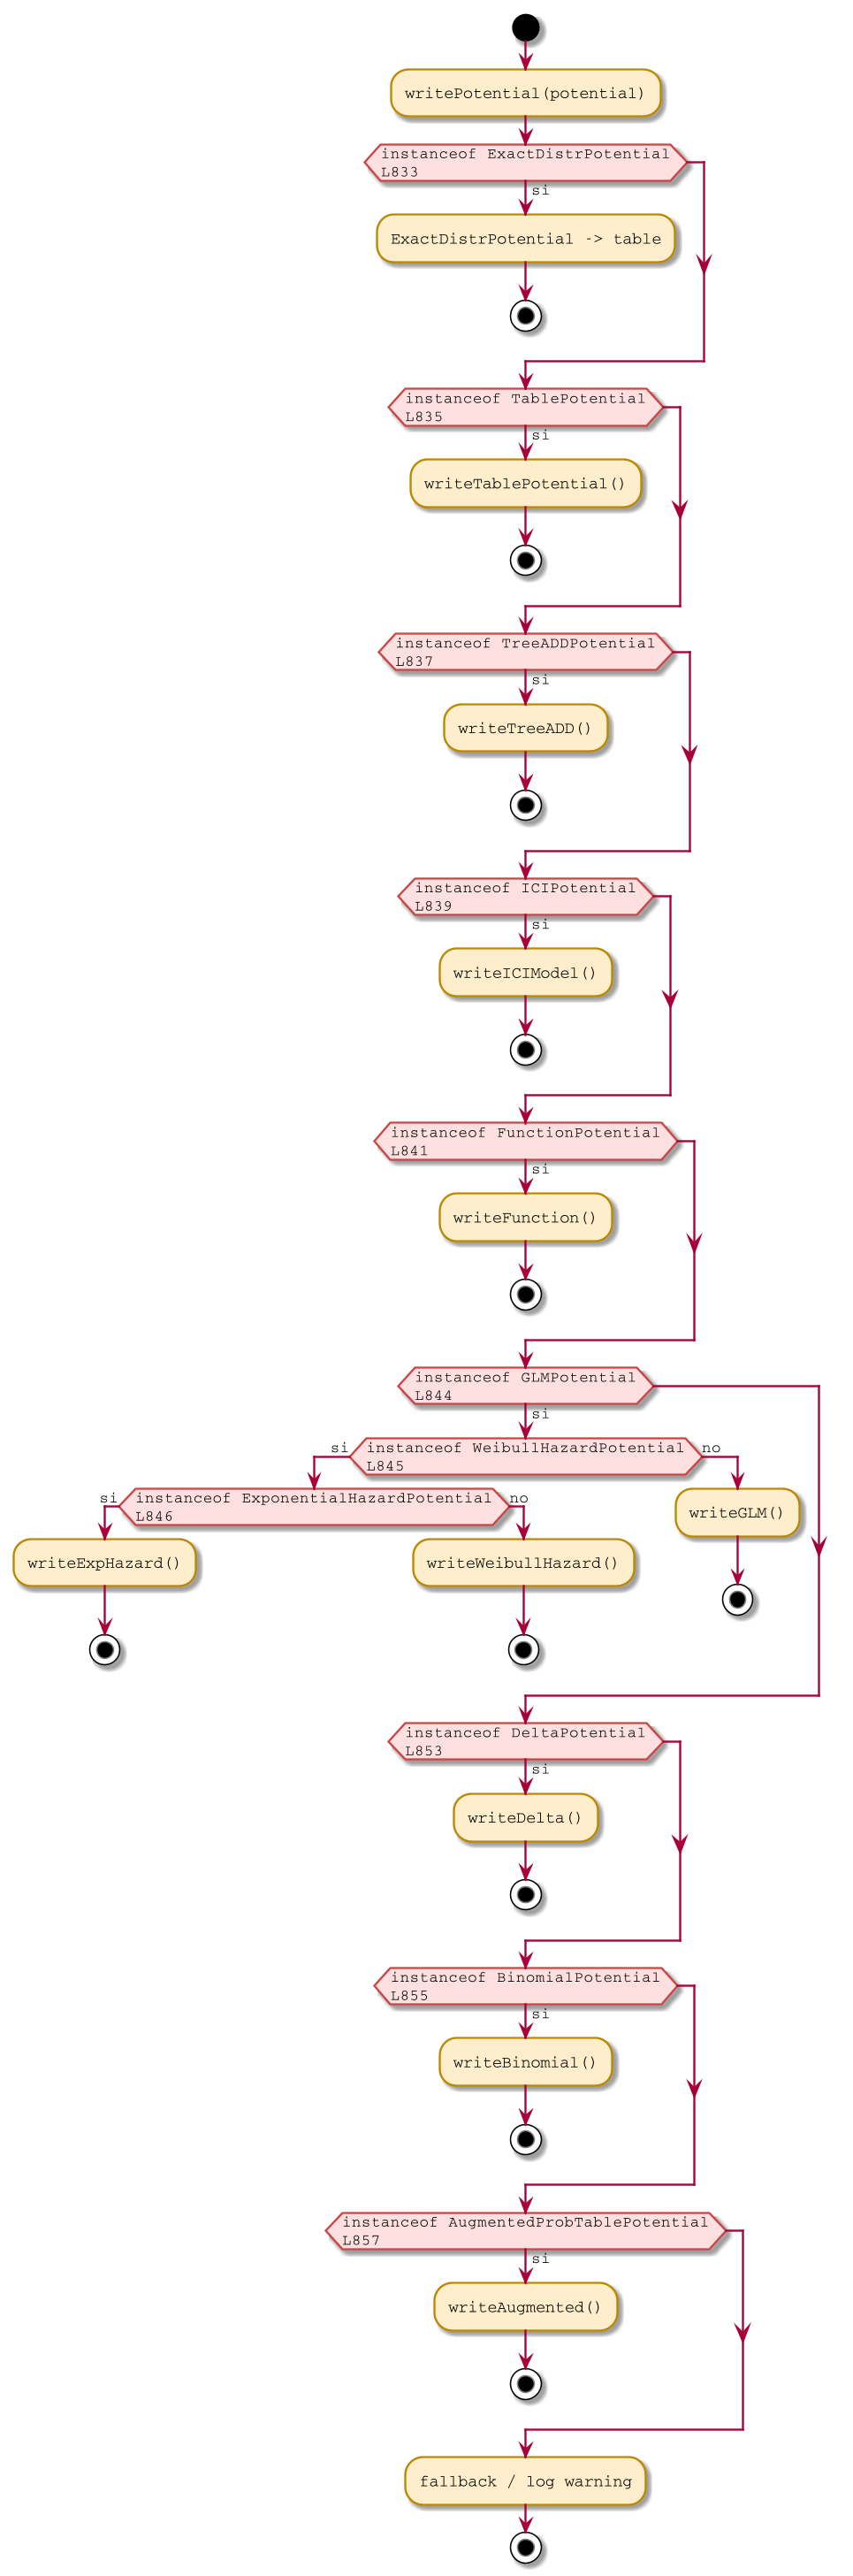
\includegraphics[width=0.78\textwidth]{cadena-instanceof-pgmx.png}
  \caption{Cadena \code{instanceof} en \code{PGMXWriter\_0\_2}. Cada nuevo
           subtipo de \code{Potential} obliga a añadir un caso aquí más en
           \code{PotentialPanelPlugin} y, si aplica, en
           \code{PGMXPotentialParsers}.}
  \label{fig:cadena-pgmx}
\end{figure}

\subsection{Uso de las fachadas \code{*PotentialOperations}}

\code{DiscretePotentialOperations} (453 líneas) y \code{PotentialOperations}
(320 líneas) son dos fachadas con dispatch redundante hacia el subpaquete
\code{operation/}. Externamente:

\begin{itemize}[leftmargin=*]
  \item \code{DiscretePotentialOperations}: 24 ficheros externos con import
        directo, \textasciitilde 80~invocaciones agregadas. Concentrado en
        \code{org.openmarkov.inference} (15 ficheros) y
        \code{org.openmarkov.core} (acciones, \code{NodeAbsorptionHandler},
        \code{Variable}, etc.).
  \item \code{PotentialOperations}: 28 ficheros externos. Mayoritariamente en
        \code{inference} (14 ficheros), \code{gui} (4),
        \code{core} (resto), \code{learning.core} (1),
        \code{integrationtests} (1).
\end{itemize}

Hay solapamiento: muchos ficheros importan ambas fachadas, lo que confirma que
no hay una división clara de responsabilidades entre ellas.

\subsection{Importaciones directas de \emph{internals} de \code{operation/}}

10 ficheros externos saltan la fachada e importan clases internas:

\begin{lstlisting}[caption={Imports directos a clases internas del subpaquete operation.}]
inference/.../timeSliceElimination/TimeSliceElimination.java:16
        AuxiliaryOperations
inference/.../dlimidevaluation/StrategyManager.java:16
        AuxiliaryOperations
inference/.../variableElimination/DecisionVariableElimination.java:17
        MaxOutVariable
gui/.../dialog/node/PotentialEditDialog.java:22
        LinkRestrictionPotentialOperations
gui/.../dialog/common/TablePotentialPanel.java:17
        LinkRestrictionPotentialOperations
gui/.../dialog/common/UnivariateDistrPotentialPanel.java:21
        LinkRestrictionPotentialOperations
gui/.../dialog/common/AugmentedProbTablePotentialPanel.java:19
        LinkRestrictionPotentialOperations
gui/.../component/LinkRestrictionValuesTable.java:20
        LinkRestrictionPotentialOperations
core/.../model/network/NodeAbsorptionHandler.java:15
        AuxiliaryOperations
core/.../action/core/SetPotentialEdit.java:12
        LinkRestrictionPotentialOperations
\end{lstlisting}

\warn{Implicación:} \code{LinkRestrictionPotentialOperations} ya es
\emph{de facto} parte de la API pública (5 clientes externos en producción).
Cualquier reorganización de \code{operation/} debe preservar esta clase como
punto público estable, o reemplazarla por una sustitución con el mismo nombre.
Lo mismo aplica para \code{AuxiliaryOperations} (3 clientes) y
\code{MaxOutVariable} (1 cliente).

\subsection{Sistema de plugins en torno a \code{Potential}}\label{sub:plugins}

Hay \emph{tres} sistemas de plugin operando en paralelo, cada uno con su
propia anotación o convención (figura~\ref{fig:plugin-systems}):

\begin{enumerate}[leftmargin=*]
  \item \textbf{\code{@PotentialType(names=\dots)}} (en \code{core}):
        descubrimiento por \code{PluginSearch} + \code{classgraph},
        consumido por \code{PotentialUtils} (\code{POTENTIALS\_BY\_NAME}).
        Sirve para serialización XML PGMX (\code{PGMXReader\_0\_2.java:1429,1445};
        \code{PGMXWriter\_0\_2.java:673,759,906};
        \code{PGMXWriter\_1\_0.java:121,197,199};
        \code{PGMXPotentialParsers.java:145,148,151};
        \code{XMLBIFReader.java:83}).
  \item \textbf{\code{@ImplementationRequirements} +
        \code{@RequiredConstructor}} (en \code{core}): contrato de
        construcción por reflexión. \code{PotentialUtils.instanciateSafely}
        (línea 86) prueba en cadena los constructores
        \code{(List, CycleLength)}, \code{(List, PotentialRole)},
        \code{(List)}, \code{(SelfClass)}.
  \item \textbf{\code{@PotentialPanelPlugin(potentialClasses=\{\dots\})}} (en
        \code{gui}): asocia \code{PotentialPanel} a un \code{Class<?
        extends Potential>}. 14 paneles concretos con la anotación
        (\code{TablePotentialPanel}: \code{\{ExactDistrPotential.class,
        TablePotential.class\}}; cada otro panel: una clase). Descubierto por
        \code{PotentialPanelManager.java:35}.
\end{enumerate}

\begin{figure}[H]
  \centering
  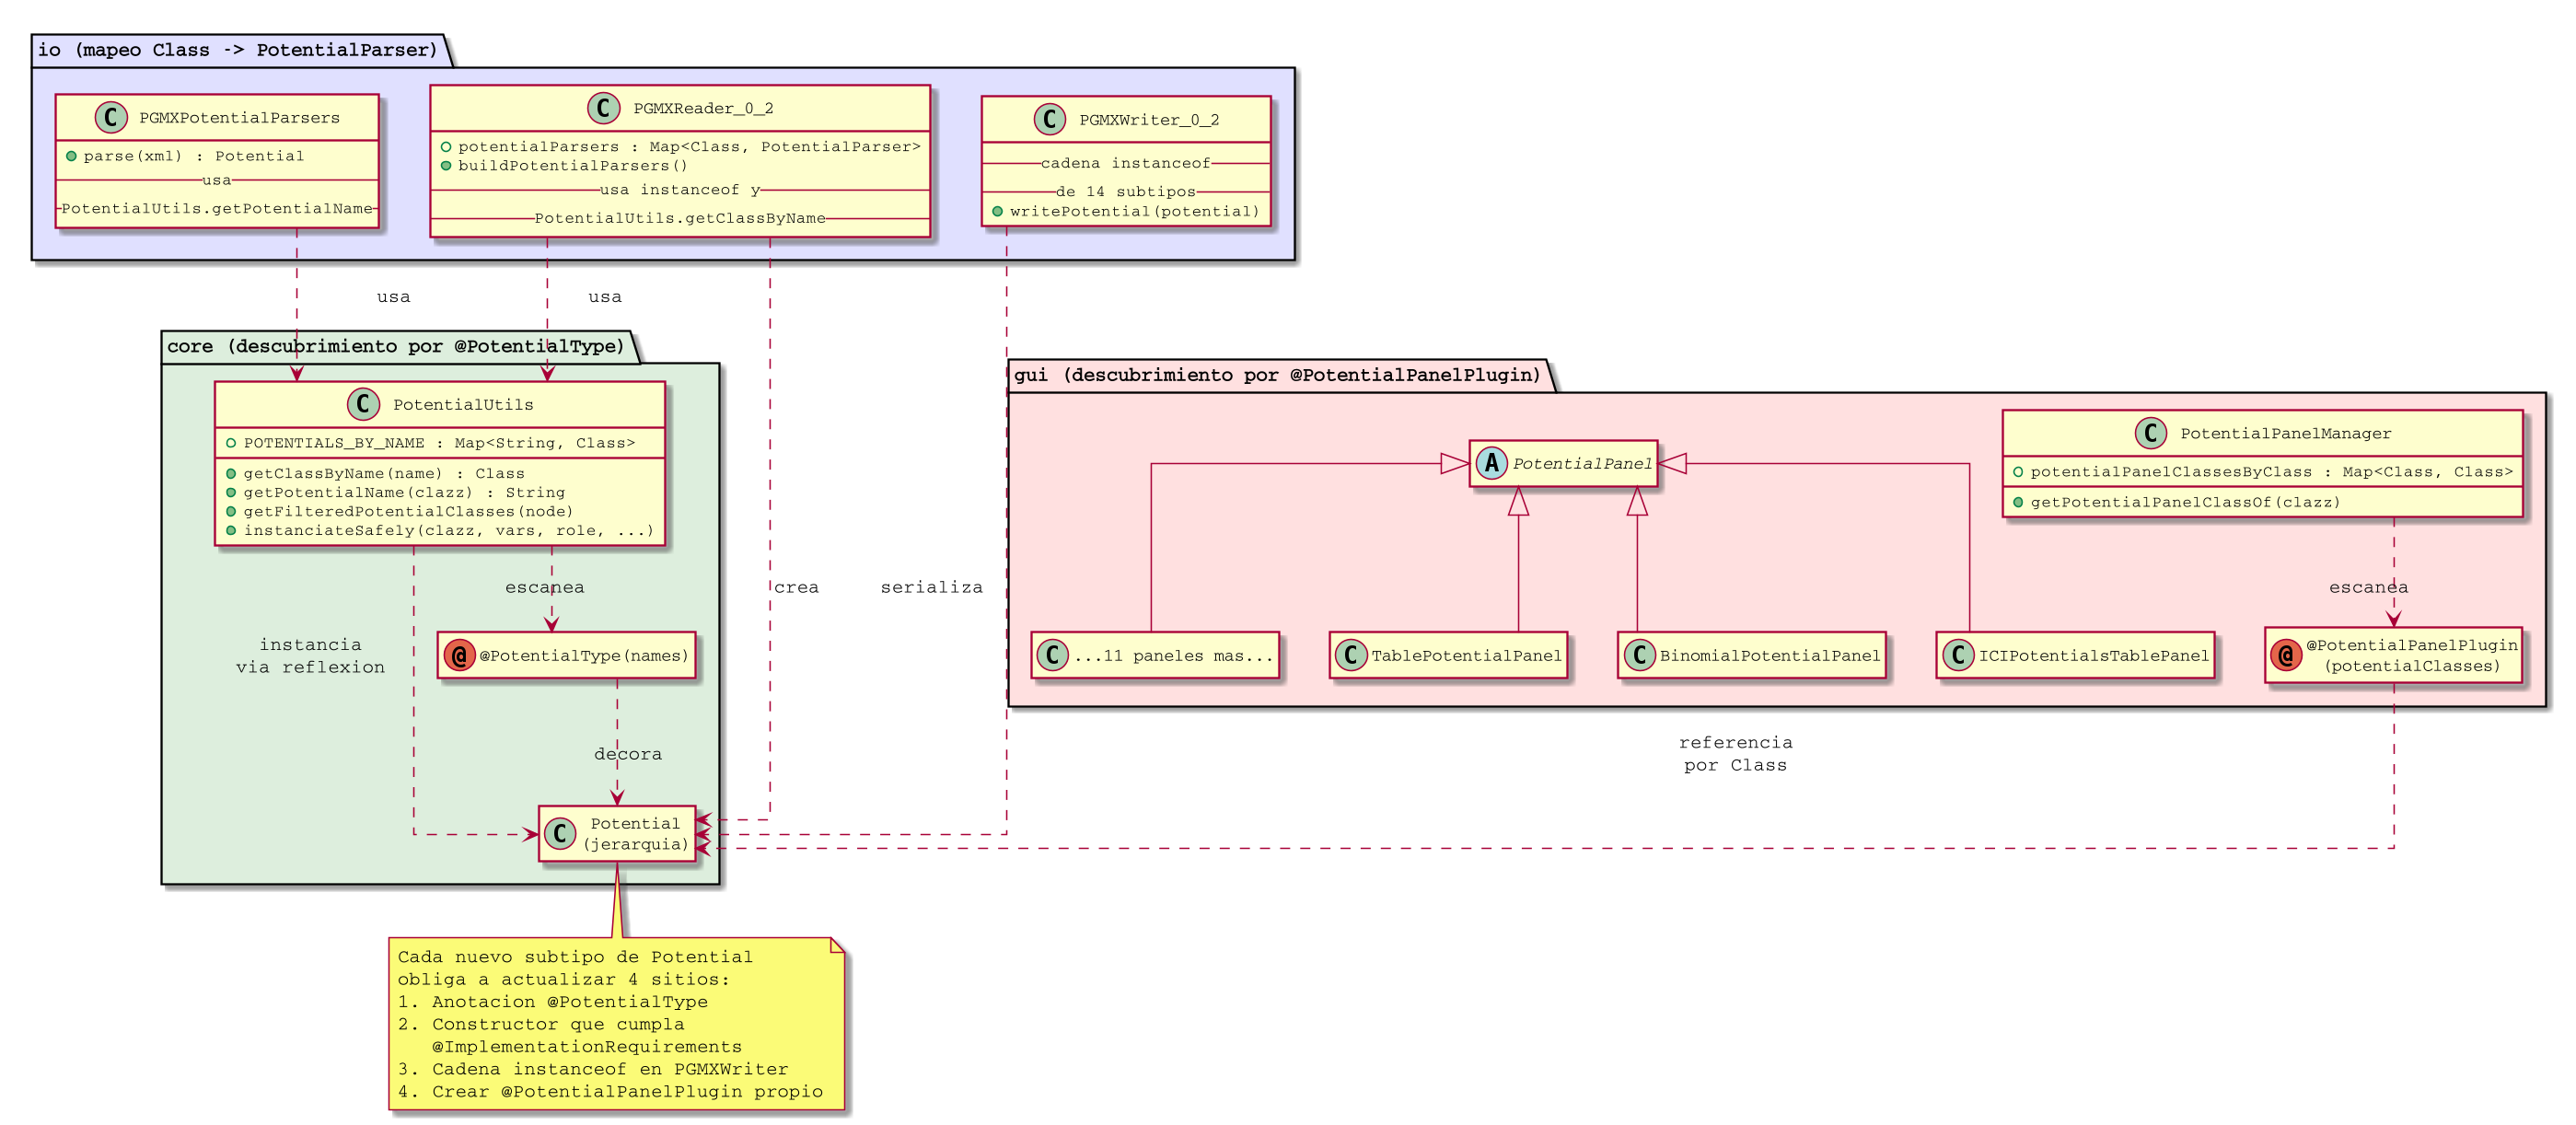
\includegraphics[width=0.95\textwidth]{plugin-systems.png}
  \caption{Tres sistemas de plugin que decoran y descubren clases de
           \code{Potential}. Añadir un nuevo subtipo obliga a tocar los tres,
           más la cadena \code{instanceof} de \code{PGMXWriter}.}
  \label{fig:plugin-systems}
\end{figure}

\subsection{Constructores invocados externamente}

Aproximadamente 539~invocaciones externas a constructores de potenciales (se
incluye producción y tests). Distribución:

\begin{center}
\begin{tabular}{lrl}
\toprule
\textbf{Módulo} & \textbf{Inst.} & \textbf{Ejemplos representativos} \\
\midrule
Tests externos                 & 194 & \code{TestNetworks.java:69}, \code{ExampleNets.java:47} \\
\code{org.openmarkov.inference}     &  61 & \code{StochasticPropagation.java:201} \\
\code{org.openmarkov.io}            &  34 & \code{ElviraParser.java:150,491,500,505}; \code{PGMXReader\_0\_2.java:1486} \\
\code{org.openmarkov.gui}           &  16 & \code{ElviraWriter.java:547}, \code{PotentialEditDialog} \\
\code{org.openmarkov.learning.core} &   1 & \code{LearningAlgorithm.java} \\
\bottomrule
\end{tabular}
\end{center}

\textbf{Tipos más instanciados}: \code{TablePotential} (\textasciitilde 220),
\code{ExactDistrPotential} (\textasciitilde 60), \code{MaxPotential}
(\textasciitilde 40), \code{MinPotential} (\textasciitilde 40),
\code{TreeADDPotential} (\textasciitilde 35), \code{SumPotential}
(\textasciitilde 25), \code{ProductPotential} (\textasciitilde 25),
\code{DeltaPotential} (\textasciitilde 15), \code{UniformPotential}
(\textasciitilde 8). Las firmas de constructor más usadas son
\code{(List<Variable>, PotentialRole)} y \code{(List<Variable>,
PotentialRole, double[])}.

\warn{Implicación:} cambios en estas firmas tienen huella muy amplia. La firma
\code{(List<Variable>, PotentialRole)} es la \emph{de facto} canónica.

\subsection{Métodos públicos de \code{Potential} invocados desde fuera}

Top de métodos por uso externo agregado:

\begin{center}
\begin{tabular}{lrl}
\toprule
\textbf{Método} & \textbf{Ficheros} & \textbf{Comentario} \\
\midrule
\code{getVariables()}       & 186 & ubicuo \\
\code{getValues()}          & 112 & lectura del array \\
\code{getValue(\dots)}      &  55 & acceso indexado \\
\code{setValues(double[])}  &  35 & GUI, learning, tests \\
\code{getProbability(\dots)}&  19 & query probabilística \\
\code{tableProject(\dots)}  &  17 & inferencia \\
\code{getCPT()}             &   9 & expansión a tabla \\
\code{getUncertainValues()} &  10 & sensibilidad \\
\code{setUncertainValues(\dots)} &  6 & sensibilidad \\
\code{setPotentialRole(\dots)}    &  5 & roles \\
\code{removeVariable(\dots)}      &  4 & ediciones \\
\code{replaceVariable(\dots)}     &  2 & ediciones \\
\code{addVariable(\dots)}         &  1 & ediciones \\
\bottomrule
\end{tabular}
\end{center}

Métodos sin uso externo significativo:
\code{sampleConditionedVariable} (0), \code{replaceNumericVariable} (0),
\code{scalePotential} directo (0), \code{reorder} directo (0),
\code{setComment} (0), \code{isAdditive} (0), \code{hasInterventions} (0),
\code{hasInterventionForDecision} (0). Estos son candidatos seguros a mover
a interfaces de capacidad o a privatizar.

\subsection{Mutadores específicos por subtipo}

Llamadas externas a setters específicos de subtipo (acotadas a producción):

\begin{itemize}[leftmargin=*]
  \item \code{ICIPotentialEdit.java:48,50,57,59} ---
        \code{setNoisyParameters(\dots)}, \code{setLeakyParameters(\dots)}
        (ediciones del modelo).
  \item \code{NodeStateEdit.java:180} ---
        \code{restrictionPotential.setValues(\dots)} para link restrictions.
  \item \code{UncertainValuesEdit.java:126,127},
        \code{UncertainValuesRemoveEdit.java:121} ---
        \code{setUncertainValues(null)} y \code{setValues(\dots)}.
  \item \code{Choice.java:52} (inferencia) --- \code{this.setValues(values)}.
  \item \code{DANFactory.java:1002,1009} ---
        \code{setValues(double[])} sobre potenciales de restricción.
\end{itemize}

\subsection{Serialización PGMX en detalle}\label{sub:pgmx}

PGMX es la fuente más sensible al rediseño. \code{PGMXReader\_0\_2}:

\begin{itemize}[leftmargin=*,itemsep=2pt]
  \item \code{PGMXReader\_0\_2.java:60} --- campo \code{public final}
        \code{Map<Class<? extends Potential>, PotentialParser>}
        \code{potentialParsers} (mapeo por \code{Class}).
  \item \code{PGMXReader\_0\_2.java:1429} --- llamada
        \code{PotentialUtils.getNames(TablePotential.class).contains(\dots)}
        que condiciona la decisión sobre rol de utilidad.
  \item \code{PGMXReader\_0\_2.java:1445} ---
        \code{PotentialUtils.getClassByName(sXmlPotentialType)}: \emph{lookup}
        dinámico de la clase a partir del XML.
  \item \code{PGMXReader\_0\_2.java:1449} ---
        comentario explícito: \emph{``Walk up the hierarchy: subclasses that
        inherit a parent's @PotentialType name.''}
  \item \code{PGMXReader\_0\_2.java:1486} ---
        \code{new TreeADDPotential(variables, topVariable, xmlRole, branches)}
        (instanciación directa).
\end{itemize}

\code{PGMXWriter\_0\_2}: cadena \code{instanceof} entre líneas 746 y 860 (ver
figura~\ref{fig:cadena-pgmx}). \code{PGMXWriter\_1\_0} replica la estrategia
con un nuevo caso para \code{UnivariateDistrPotential} en línea 197--199 y 238.

\warn{Implicación:} la serialización PGMX es un contrato de fichero. Cualquier
renombrado de clase, anotación o enum (en particular
\code{PotentialRole.UNSPECIFIED} $\to$ \code{UTILITY}) requiere mantener
compatibilidad de \emph{lectura} con redes existentes.

\subsection{GUI: ediciones, paneles y mutaciones}

\subsubsection*{Sistema de paneles}

14 \code{PotentialPanel} concretos en \code{org.openmarkov.gui/.../dialog/common/}
y \code{dialog/treeadd/}, cada uno anotado con
\code{@PotentialPanelPlugin(potentialClasses=\dots)} (ver
sección~\ref{sub:plugins}). \code{TablePotentialPanel} es el único que
declara dos clases (\code{TablePotential.class} y
\code{ExactDistrPotential.class}); el resto, una sola.

\subsubsection*{Ediciones GUI}

En \code{org.openmarkov.gui/src/main/java/org/openmarkov/gui/action/}:
\code{TablePotentialValueEdit}, \code{ICITablePotentialValueEdit},
\code{AugmentedPotentialValueEdit}, \code{LinkRestrictionPotentialValueEdit}.
Estas son \code{PNEdit} subclases que aplican (y deshacen) cambios in-place
sobre el potencial. La mutación en
\code{TablePotentialValueEdit.java:162} es:

\begin{lstlisting}[caption={Mutación in-place vía \code{getValues()} en una edición.}]
tablePotential.getValues()[potentialSelected] = newValue;
\end{lstlisting}

\subsubsection*{Lectura para visualización}

\code{ValuesTable.java:710,723,729} y
\code{TraceTemporalEvolutionDialog.java:514,536,789,1395,1398,1473,1477}
leen \code{getValues()[\dots]} para pintar tablas y trazas.
\code{InferencePresenter.java:66} hace
\code{individualProbabilities.get(variable).getValues()[0]} para barras de
probabilidad por estado.

\warn{Implicación:} envolver \code{getValues()} en una vista de sólo lectura
es seguro para \emph{lectura} (la mayor parte de los 315 sitios), pero el
canal de mutación in-place desde la GUI requiere un punto de actualización
explícito (\code{setValueAt(idx, double)} o
\code{withValue(idx, double)} si vamos a inmutabilidad).

\subsection{Tests externos}

Tests que crean potenciales o inspeccionan su estructura interna:

\begin{itemize}[leftmargin=*,itemsep=2pt]
  \item \code{org.openmarkov.inference/src/test/.../TestNetworks.java:69--228},
        \code{ExampleNets.java:47--225} --- construcción de redes con
        constructores públicos.
  \item \code{org.openmarkov.io/src/test/.../PGMXReaderWriterTest.java:95,97,159};
        \code{ElviraWriterTest.java:81--110}; \code{Util.java:38--108}.
  \item \code{org.openmarkov.integrationtests/src/test/.../inference/heuristics/Tools.java:70}
        --- acceso a \code{stp.strategyTrees}.
  \item \code{org.openmarkov.integrationtests/src/test/.../io/PGMXReadersTest.java:40,43,56,57,65}
        --- conjunto \code{POTENTIALS\_WITHOUT\_PGMX\_REPRESENTATION} con
        clases excluidas; carga dinámica de \code{SDAGStrategyTree} por nombre.
  \item \code{org.openmarkov.integrationtests/.../gui/AllPotentialsHaveAPanel.java:15,21}
        --- prueba que todo \code{Potential} descubierto por \code{PluginSearch}
        tiene un \code{PotentialPanel} asociado.
  \item \code{org.openmarkov.stochasticPropagationOutput/src/test/.../ExampleNets.java:47--225}
        --- mismas construcciones que en inference tests.
\end{itemize}

Estos tests dependen sobre todo de constructores públicos y getters; \emph{no}
asumen acceso directo al \code{double[]} salvo en accesos de lectura.

\subsection{Resumen agregado por módulo}

La figura~\ref{fig:acoplamiento} resume el grado de acoplamiento por módulo
externo, y la tabla~\ref{tab:acoplamiento} cuantifica los puntos calientes.

\begin{figure}[H]
  \centering
  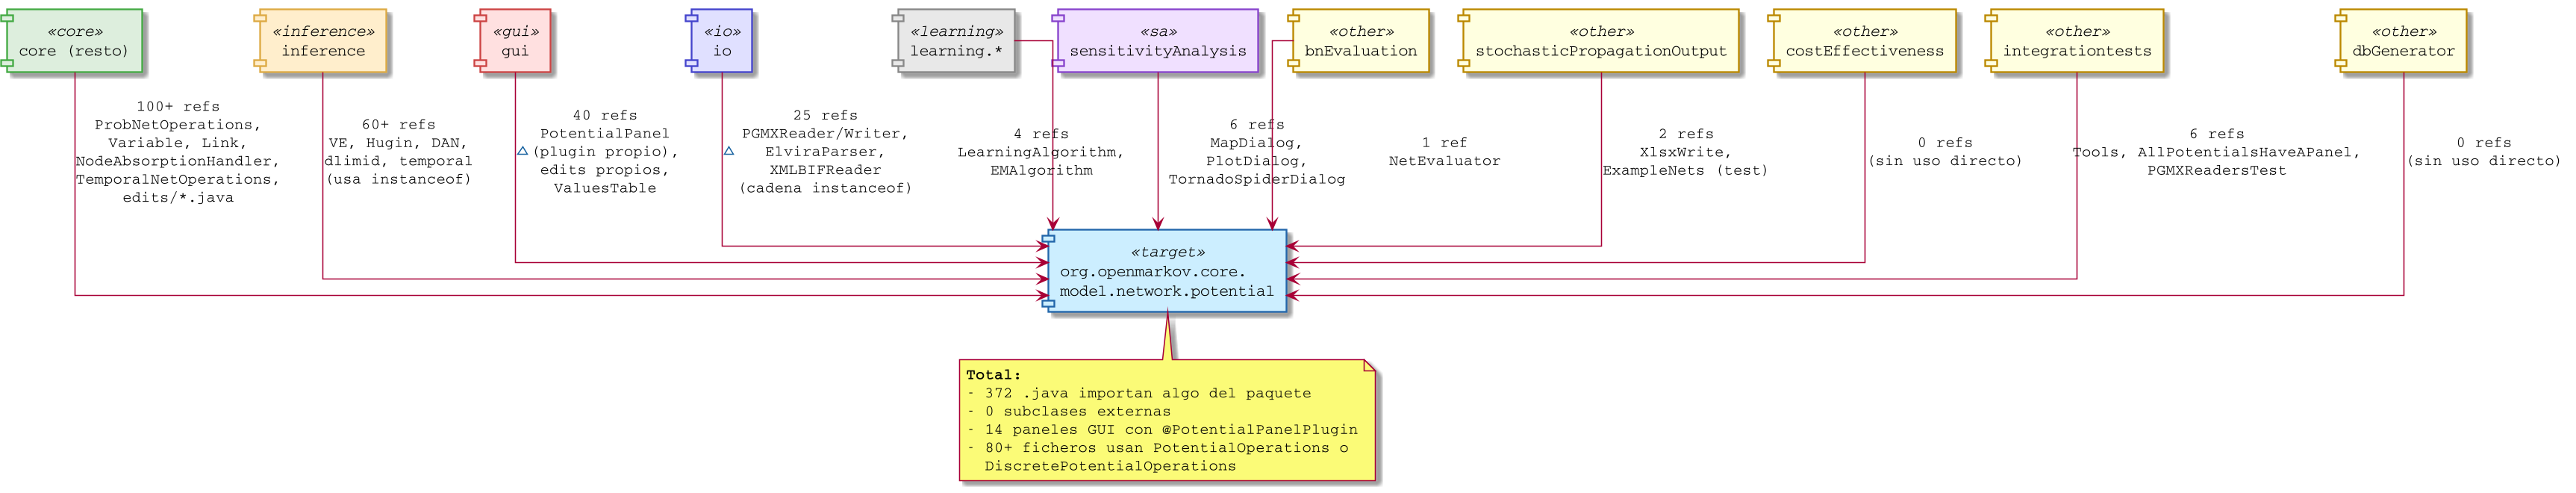
\includegraphics[width=0.95\textwidth]{acoplamiento-modulos.png}
  \caption{Acoplamiento de módulos externos al paquete \code{potential}.}
  \label{fig:acoplamiento}
\end{figure}

\begin{table}[H]
\centering
\scriptsize
\setlength{\tabcolsep}{3pt}
\begin{tabular}{lcccclp{4.2cm}}
\toprule
\textbf{Módulo} & \textbf{Refs} & \textbf{Constr.} &
\textbf{instanceof} & \textbf{Mutadores} & \textbf{Clientes principales} & \textbf{Acoplamiento dominante} \\
\midrule
core (resto)                 & alto  & 100+ & $\sim$15 & 14 & ProbNetOps, Variable, edits   & profundo (\code{.uncertainValues}) \\
inference                    & alto  &  61  & $\sim$25 &  4 & VE, Hugin, DAN                & \code{instanceof} + \code{.strategyTrees} \\
gui                          & alto  &  16  & $\sim$30 &  6 & PotentialPanel + edits        & cadena \code{instanceof} + plugin \\
io                           & alto  &  34  & $\sim$20 &  2 & PGMX + Elvira                 & cadena \code{instanceof} en writers \\
learning.core / .algorithm   & medio &   2  &    0     &  0 & LearningAlgorithm, EM         & \code{getValues()[i]} \\
sensitivityAnalysis          & medio &   0  &    0     &  0 & MapDialog, Plot, Tornado      & \code{getValues()[i]} (lectura) \\
bnEvaluation                 & bajo  &   0  &    0     &  0 & NetEvaluator                  & \code{getValues()[0]} (lectura) \\
stochasticPropagationOutput  & bajo  &   2  &    0     &  0 & XlsxWrite                     & \code{getValues()[i]} (lectura) \\
costEffectiveness            & nulo  &   0  &    0     &  0 & ---                           & --- \\
dbGenerator                  & nulo  &   0  &    0     &  0 & ---                           & --- \\
integrationtests             & medio &   2  & $\sim$5  &  0 & PGMXReadersTest, Tools        & \code{strategyTrees} (test) \\
\bottomrule
\end{tabular}
\caption{Resumen de acoplamiento por módulo. ``Refs'' es cualitativo
         (alto/medio/bajo); las columnas numéricas cuentan ficheros distintos
         en producción.}
\label{tab:acoplamiento}
\end{table}

\section{Replanteamiento de las opciones de refactor}

A continuación se reformulan las opciones del informe previo a la luz de los
datos del análisis cruzado. Cada opción incluye \emph{huella esperada en
módulos externos} y \emph{condicionantes} concretos.

\subsection{Opción A --- Higiene local} (riesgo bajo)

\begin{itemize}[leftmargin=*]
  \item Eliminar \code{operation/Util.java} (formato/paths, no propio del
        paquete) $\to$ mover a \code{org.openmarkov.java}.
  \item Borrar \textasciitilde 130~líneas de código comentado en
        \code{MaxOutVariable.java:172--304}; comentarios obsoletos en
        \code{TablePotential}, \code{TreeADDPotential}, \code{Potential}.
  \item Añadir \code{hashCode()} consistente con \code{equals()} en
        \code{Potential}, \code{TablePotential},
        \code{Uncertain\-Table\-Potential},
        \code{StrategicTablePotential}.
  \item Hacer null-safe \code{Potential.equals()} y \code{TablePotential.equals()}.
  \item Hacer \code{Potential.properties} privado con getter/setter
        (\good{huella externa nula}: 0 accesos directos).
  \item Documentar \code{Potential.setPotentialRole} o restringirlo a
        \code{package-private}.
\end{itemize}

\textbf{Huella externa estimada:} 0 ficheros producción tocados, salvo el
movimiento de \code{Util.java} (huella nula porque sólo se usa internamente,
\emph{verificar antes}).

\subsubsection*{Pros}
\begin{itemize}[leftmargin=*]
  \item Riesgo prácticamente nulo. Las pruebas property-based existentes
        (memoria del proyecto, plan \code{project\_test\_plan.md}) cubren
        \code{equals/hashCode} y mutaciones.
  \item Mejora robustez (NPE en \code{equals}) sin coste arquitectónico.
\end{itemize}

\subsubsection*{Contras}
\begin{itemize}[leftmargin=*]
  \item No resuelve los problemas estructurales (defaults que lanzan, plugins
        a tres bandas, etc.).
  \item El cambio de \code{hashCode} obliga a verificar uso en colecciones
        \code{HashMap}/\code{HashSet}; es muy improbable que \code{Potential}
        se use como clave (no aparecería en mapas) pero es disciplina
        obligatoria revisarlo.
\end{itemize}

\subsection{Opción B --- Completar la migración a interfaces de capacidad}
(riesgo medio, recompensa alta)

Eliminar de \code{Potential} los \emph{defaults} que lanzan
\code{UnsupportedOperationException} y dejar que cada capacidad sea
verdaderamente opcional. La forma objetivo es la
figura~\ref{fig:objetivo-fase2}.

\begin{figure}[H]
  \centering
  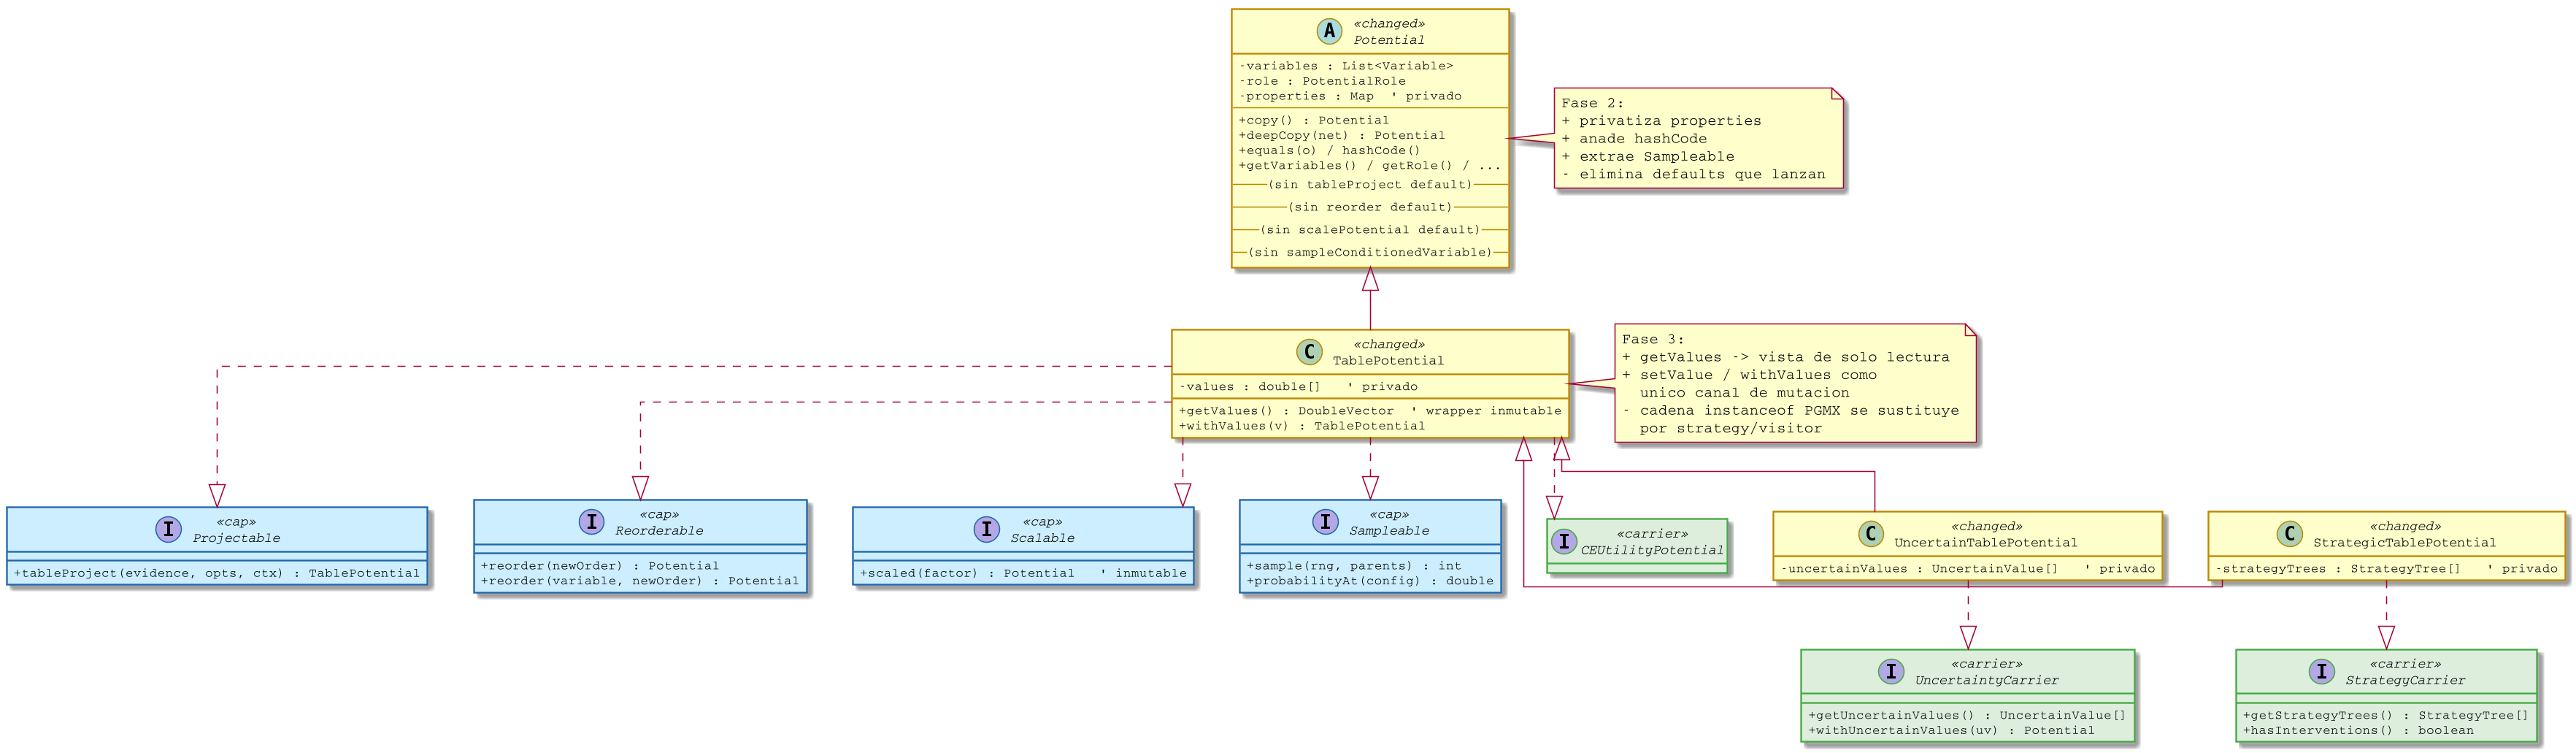
\includegraphics[width=\textwidth]{objetivo-fase2.png}
  \caption{Estado objetivo tras la fase 2: capacidades canónicas, sin
           \emph{defaults} que lanzan, campos privados y wrappers de mutación
           explícitos.}
  \label{fig:objetivo-fase2}
\end{figure}

\textbf{Pasos concretos:}

\begin{enumerate}[leftmargin=*]
  \item Promover \code{Projectable.tableProject} a la única firma oficial.
        Eliminar
        \code{Potential.tableProject(EvidenceCase, InferenceOptions, List<TablePotential>)}.
        Para cubrir el caso usado por \code{ProductPotential},
        \code{SumPotential}, \code{ICIPotential}, introducir
        \code{ProjectionContext} que envuelve la lista de potenciales
        ya proyectados.
  \item Crear \code{Sampleable} con \code{sampleConditionedVariable} y
        \code{probabilityAt}. Mover el default que devuelve 0 fuera de
        \code{Potential}.
  \item Borrar \code{Potential.scalePotential} y \code{Potential.reorder(\dots)}.
        Las \textasciitilde 12~implementaciones vacías o que devuelven
        \code{copy()} se eliminan.
  \item Privatizar \code{StrategicTablePotential.strategyTrees} y
        \code{Uncertain\-Table\-Potential.uncertainValues}; exponer vía
        \code{StrategyCarrier.getStrategyTrees()},
        \code{StrategyCarrier.withStrategyTrees(\dots)}, equivalentes para
        \code{UncertaintyCarrier}.
\end{enumerate}

\textbf{Huella externa estimada (verificada):}

\begin{itemize}[leftmargin=*]
  \item \bad{2 sitios} de escritura directa a
        \code{strategicTablePotential.strategyTrees} en
        \code{VEOptimalIntervention.java:85,86}.
  \item \bad{6 sitios} de lectura/escritura a
        \code{uncertainPotential.uncertainValues} en
        \code{ProbNetOperations.java} (4) y
        \code{SystematicSampling.java} (2).
  \item \bad{5 sitios} de tests con escritura literal en
        \code{SensitivityAnalysisFactory.java}.
  \item Inferencia y GUI siguen invocando \code{tableProject} a través de las
        firmas existentes.
\end{itemize}

Total: \textbf{$\sim$15 sitios externos a tocar}.

\subsubsection*{Pros}
\begin{itemize}[leftmargin=*]
  \item Resuelve el problema documentado en
        \code{Projectable.java:25}: la base ya no miente sobre las capacidades
        que ofrece.
  \item Las property-based ya existentes para
        \code{StrategicTablePotential} (memoria del proyecto: 7~tests en
        \code{StrategicTablePotentialTest.java}) actúan como red de seguridad.
  \item No hay subclases externas (sección~\ref{sub:no-subclasses}), así que
        ningún plugin de tercero rompe.
\end{itemize}

\subsubsection*{Contras}
\begin{itemize}[leftmargin=*]
  \item 15+ sitios producción a tocar, distribuidos entre \code{core},
        \code{inference} y \code{tests}. Necesita una \emph{property} previa
        que ancle el flujo \code{ProbNet\-Operations} con incertidumbre antes
        del cambio.
  \item Cambio de firma en \code{Projectable.tableProject} obliga a actualizar
        17 clientes externos identificados.
\end{itemize}

\subsection{Opción C --- Renombrar \code{PotentialRole.UNSPECIFIED} a
\code{UTILITY}} (riesgo medio, principalmente PGMX)

\textbf{Huella externa:}

\begin{itemize}[leftmargin=*]
  \item Lectores/escritores PGMX (\code{PGMXReader\_0\_2.java:1429},
        \code{PGMXWriter\_0\_2.java:746}, \code{PGMXWriter\_1\_0}): mapeo
        \code{role="utility" $\leftrightarrow$ UNSPECIFIED} debe convertirse
        en \code{role="utility" $\leftrightarrow$ UTILITY} con compatibilidad
        de \emph{lectura} para ficheros antiguos (que ya escriben
        \code{utility}).
  \item Cualquier \code{case UNSPECIFIED} en producción: estimado en
        \textasciitilde 30 sitios totales (entre el paquete y consumidores
        directos como \code{TableProb\-Operations}, \code{ProbNetWriter},
        \code{InferenceManager}).
\end{itemize}

\subsubsection*{Pros}
\begin{itemize}[leftmargin=*]
  \item Modelo conceptualmente honesto. Reduce comentarios del tipo ``esto
        es utility en realidad''.
  \item Permite eliminar duplicación con \code{isAdditive} (que actualmente
        lo redunda).
\end{itemize}

\subsubsection*{Contras}
\begin{itemize}[leftmargin=*]
  \item Compatibilidad de archivos PGMX existentes; si se rompe la lectura,
        ningún test sobre \code{*.xml} legacy en
        \code{src/test/resources/nets/} pasaría.
  \item Riesgo de regresión silenciosa en flujos de utilidad (donde
        \code{UNSPECIFIED} es el marcador).
\end{itemize}

\subsection{Opción D --- Aplanar la fachada de operaciones}
(riesgo medio, sobre todo \emph{churn})

Mantener una sola fachada (probablemente \code{PotentialOperations}) y
suprimir \code{DiscretePotentialOperations} (o viceversa). Reorganizar
\code{operation/} en submódulos temáticos (\code{arithmetic/},
\code{elimination/}, \code{factory/}, \code{transform/}).

\textbf{Huella externa:} 24~ficheros importan
\code{DiscretePotentialOperations}, 28~importan \code{PotentialOperations}.
Si se conserva \code{PotentialOperations}, hay que migrar 24~importaciones.

\subsubsection*{Pros}
\begin{itemize}[leftmargin=*]
  \item Una única fachada elimina la decisión ``¿qué fachada uso aquí?''.
  \item Reorganizar \code{operation/} reduce la sensación de paquete plano
        con 15~ficheros heterogéneos.
\end{itemize}

\subsubsection*{Contras}
\begin{itemize}[leftmargin=*]
  \item 24+ ficheros con \code{import} cambiado: ruido en \code{git blame}.
  \item Hay que decidir qué hacer con
        \code{LinkRestrictionPotentialOperations} (5 clientes externos,
        \code{de facto} público) y \code{AuxiliaryOperations} (3 clientes):
        no se pueden ocultar.
\end{itemize}

\subsection{Opción E --- Unificar las firmas de \code{tableProject}}
(riesgo medio, queda incluida en la Opción B)

Dejar una única firma \code{tableProject(EvidenceCase, InferenceOptions, ProjectionContext)}.
Sólo \code{ProductPotential.tableProject:86},
\code{SumPotential.tableProject:85} y \code{ICIPotential.tableProject:201}
necesitan el contexto. Esto resuelve la duplicación de
\code{Potential.tableProject(\dots)} con \code{Projectable.tableProject(\dots)}.

\textbf{Huella externa:} \textbf{17~ficheros} fuera del paquete invocan
alguna sobrecarga de \code{tableProject}. La migración es mecánica: añadir
\code{ProjectionContext.empty()} en los call-sites.

\subsection{Opción F --- Composición sobre herencia (Strategic / Uncertain
como decoradores)} (riesgo alto)

Reformular \code{StrategicTablePotential} y \code{UncertainTablePotential}
como decoradores (\code{TablePotential delegate + state}) en lugar de
subclases. Permite combinaciones (uncertain $\times$ strategic) que hoy son
imposibles, citadas como caso ``raro no soportado'' en
\code{TreeADDPotential.blendPotentials} (líneas 622--624).

\textbf{Huella externa estimada:} 317 ficheros referencian
\code{TablePotential}, \code{Uncertain\-Table\-Potential} o
\code{Strategic\-Table\-Potential}. La mayoría no necesitan cambio si:

\begin{itemize}[leftmargin=*]
  \item \code{TablePotential} mantiene la misma API pública.
  \item Los decoradores \emph{son} \code{TablePotential} (vía interfaz, no por
        herencia).
  \item Las cadenas \code{instanceof} en
        \code{PGMXWriter\_0\_2.java:746--860} pasan a usar las interfaces
        \code{StrategyCarrier} / \code{UncertaintyCarrier}.
\end{itemize}

Aún así, los \textbf{17~accesos directos} a campos públicos
(\code{strategyTrees}, \code{uncertainValues}) en código externo ya analizados
(sección~\ref{sub:fields}) hay que migrarlos.

\subsubsection*{Pros}
\begin{itemize}[leftmargin=*]
  \item Resuelve el caso ``uncertain $\times$ strategic'' anotado en
        \code{TreeADDPotential.java:622--624}.
  \item Facilita futuras capacidades opcionales sin explosión de subclases.
\end{itemize}

\subsubsection*{Contras}
\begin{itemize}[leftmargin=*]
  \item Cambio profundo. Coste de allocation por decorador.
  \item Los plugins GUI (\code{@PotentialPanelPlugin(potentialClasses=\dots)})
        están atados por literal de clase; el panel de
        \code{StrategicTablePotential} no existe (hereda de
        \code{TablePotentialPanel}), pero conviene revisar.
\end{itemize}

\subsection{Opción G --- Inmutabilidad estricta} (riesgo muy alto)

Eliminar \code{setValues}, \code{setUniform}, \code{scalePotential},
\code{setUncertainValues} y todas las mutaciones in-place. Foco principal de
mutación según el análisis cruzado:

\begin{itemize}[leftmargin=*]
  \item 7 escrituras a \code{getValues()[i]} en producción
        (sección~\ref{sub:fields}).
  \item 63 invocaciones externas a \code{setValues}, \code{setUncertainValues},
        \code{setNoisyParameters}, \code{setLeakyParameters}, etc. Concentradas
        en \code{org.openmarkov.core/.../action/} (ediciones PNEdit) y
        \code{DANFactory}.
  \item Edición GUI \code{TablePotentialValueEdit.java:162} es el único
        \emph{write-back} desde la GUI.
\end{itemize}

\subsubsection*{Pros}
\begin{itemize}[leftmargin=*]
  \item Thread-safety; razonamiento simplificado; cache seguro.
  \item Previene casos como
        \code{TablePotential.tableProject:191--193}, donde se devuelve
        \code{this} sin clonar el array (aliasing accidental).
\end{itemize}

\subsubsection*{Contras}
\begin{itemize}[leftmargin=*]
  \item Las ediciones \code{PNEdit} dependen de mutar y revertir
        in-place. Migrar a ``edit + replace potential in node'' afecta
        \code{ProbNet}, \code{Node}, \code{PNESupport} (semántica de undo).
  \item Coste de allocation puede impactar redes grandes: cada multiplicación
        ya devuelve nuevas instancias, pero \code{normalize}, \code{setUniform}
        y \code{scalePotential} optimizan in-place hoy.
  \item \emph{No es prerequisito} para Opciones A--F. Postergable.
\end{itemize}

\subsection{Opción H --- Sustituir cadena \code{instanceof} de PGMX por
\emph{strategy/visitor}} (riesgo medio, valor alto)

La cadena \code{PGMXWriter\_0\_2.java:746--860} y su gemela en
\code{PGMXWriter\_1\_0} crecen cada vez que se añade un subtipo. Posibles
soluciones:

\begin{itemize}[leftmargin=*]
  \item \emph{Strategy registrada por \code{Class}}, simétrica al mapa
        \code{potentialParsers} que ya existe en
        \code{PGMXReader\_0\_2.java:60} para lectura.
  \item \emph{Visitor} con \code{Potential.accept(PotentialVisitor)}; es
        intrusivo en la base.
  \item \emph{Pattern matching switch} (Java 21+): mantener la cadena pero
        en una expresión \code{switch} más limpia, sin cambiar la API.
\end{itemize}

\textbf{Huella externa:} sólo \code{org.openmarkov.io}. La estructura de
escritura del XML PGMX no cambia.

\subsubsection*{Pros}
\begin{itemize}[leftmargin=*]
  \item Cada nuevo subtipo registra su escritor en un punto único.
  \item Simetría con la lectura: ambas direcciones consultan un mapa.
\end{itemize}

\subsubsection*{Contras}
\begin{itemize}[leftmargin=*]
  \item \code{org.openmarkov.io} crece en infraestructura.
  \item Si se eligen ``strategies registradas por classgraph'', se añade un
        cuarto sistema de plugin a los tres ya existentes.
\end{itemize}

\subsection{Comparativa de opciones}

\begin{table}[H]
\centering
\scriptsize
\setlength{\tabcolsep}{4pt}
\begin{tabular}{p{4cm}lllllc}
\toprule
\textbf{Opción} & \textbf{Riesgo} & \textbf{Esfuerzo} &
\textbf{Externa} & \textbf{Rev.} & \textbf{Beneficio} & \textbf{Prereq.} \\
\midrule
A. Higiene local                       & bajo     & 1--2 ses. & $\sim$0  & sí      & medio & --- \\
B. Capacidades canónicas               & medio    & 3--4 ses. & $\sim$15 & sí      & alto  & A   \\
C. \code{UNSPECIFIED $\to$ UTILITY}    & medio    & 2 ses.    & $\sim$30 & no\textsuperscript{$\dagger$} & medio & A \\
D. Aplanar fachadas                    & medio    & 2 ses.    & 24       & sí      & medio & --- \\
E. Unificar \code{tableProject}        & medio    & 1--2 ses. & 17       & sí      & medio & B   \\
F. Composición Strategic / Uncertain   & alto     & 6+ ses.   & $\sim$25 & parcial & alto  & B   \\
G. Inmutabilidad estricta              & muy alto & 10+ ses.  & 70+      & no      & alto  & B,F \\
H. Strategy en \code{PGMXWriter}       & medio    & 2 ses.    & 0 prod.  & sí      & medio & --- \\
\bottomrule
\end{tabular}
\caption{Comparativa. ``Externa'' = ficheros no-paquete a tocar (estimado).
         \textsuperscript{$\dagger$}~no reversible \emph{a nivel de fichero
         PGMX} si rompemos compatibilidad de lectura.}
\end{table}

\section{Plan de acción por fases}\label{sec:plan}

Cinco fases incrementales, pensadas para ser cada una un PR autónomo con
verde en \code{mvn install} y todas las property-based ya existentes.

\subsection{Fase 0 --- Anclar el comportamiento actual con properties}

\textbf{Objetivo:} ampliar la red de tests antes de tocar la base. Se
inspira en la fase 0 de \code{ProbNet refactoring} (memoria del proyecto:
\code{project\_probnet\_refactoring.md}), que pasó de 37\% a $\sim$80\% de
cobertura antes del refactor.

\begin{itemize}[leftmargin=*]
  \item Property-based para \code{Potential.equals}/\code{hashCode} (con
        ejemplos de subtipos heterogéneos).
  \item Property-based para \code{deepCopy}: el grafo de variables se reasigna
        al \code{copyNet}; ningún campo queda ``apuntando'' al original.
  \item Property-based para \code{DiscretePotentialOperations.multiplyAndMarginalize}
        con potenciales que mezclan \code{StrategicTablePotential} y
        \code{TablePotential} (intervenciones se preservan).
  \item Property-based para
        \code{ProbNetOperations.proyect-uncertain} (línea 618--634), que es
        el único punto productivo con escritura externa a
        \code{uncertainValues}.
\end{itemize}

\textbf{Criterios de aceptación:} todas las nuevas properties pasan en la
rama actual sin tocar código de producción.

\textbf{Huella externa:} 0.

\subsection{Fase 1 --- Higiene local (Opción A)}

\textbf{Objetivo:} cerrar inconsistencias menores antes de cualquier cambio
de API.

\begin{itemize}[leftmargin=*]
  \item Mover \code{operation/Util.java} a \code{org.openmarkov.java}.
  \item Borrar código comentado en \code{MaxOutVariable},
        \code{TablePotential}, \code{Potential},
        \code{TreeADDPotential}.
  \item Añadir \code{hashCode()} consistentes y \code{Objects.equals}-style
        null-safety.
  \item Privatizar \code{Potential.properties}, exponer vía getter/setter.
  \item Auditar \code{Potential.setPotentialRole} y restringir su visibilidad.
\end{itemize}

\textbf{Criterios de aceptación:} property-based de la Fase 0 verdes;
\code{mvn install -DskipTests=false} verde; ninguna firma pública alterada
salvo \code{properties} (de campo a getter --- 0 clientes externos).

\textbf{Huella externa:} 0 modificaciones esperadas.

\subsection{Fase 2 --- Capacidades canónicas (Opción B + Opción E)}

\textbf{Objetivo:} eliminar los \emph{defaults} que lanzan en
\code{Potential}; unificar \code{tableProject}; privatizar \code{strategyTrees}
y \code{uncertainValues}. Estado objetivo en
figura~\ref{fig:objetivo-fase2}.

\textbf{Subfases:}

\begin{enumerate}[leftmargin=*]
  \item[\textbf{2a}] Introducir \code{ProjectionContext}; migrar las
        17~invocaciones externas de \code{tableProject(\dots)} a la firma
        única; eliminar la sobrecarga con \code{List<TablePotential>}.
  \item[\textbf{2b}] Crear \code{Sampleable}; migrar \code{sampleConditionedVariable}
        y \code{getProbability}. Borrar el default 0 de \code{Potential.getProbability}.
  \item[\textbf{2c}] Privatizar \code{StrategicTablePotential.strategyTrees}.
        Modificar \code{VEOptimalIntervention.java:85,86} y
        \code{Tools.java:70} (3 sitios).
  \item[\textbf{2d}] Privatizar \code{UncertainTablePotential.uncertainValues}.
        Modificar \code{ProbNetOperations.java:618--634},
        \code{SystematicSampling.java:150,162} y los 5 sitios de tests
        (\code{SensitivityAnalysisFactory}). 11 sitios.
  \item[\textbf{2e}] Borrar \code{Potential.scalePotential},
        \code{Potential.reorder(\dots)}. Limpiar las
        \textasciitilde 12~implementaciones vacías.
\end{enumerate}

\textbf{Criterios de aceptación por subfase:} \code{mvn install} verde,
property-based de Fase~0 verdes, tests de inferencia
(\code{InferenceAlgorithmIDTest}, \code{DANTest}) verdes.

\textbf{Huella externa total:} \textbf{$\sim$15--20 ficheros producción
modificados}, distribuidos en \code{core}, \code{inference}, tests.

\subsection{Fase 3 --- Strategy en \code{PGMXWriter} (Opción H)}

\textbf{Objetivo:} eliminar la cadena \code{instanceof} de
\code{PGMXWriter\_0\_2.java:746--860} y su gemela en \code{PGMXWriter\_1\_0}.

\begin{itemize}[leftmargin=*]
  \item Crear \code{PotentialWriterStrategy} con un mapa
        \code{Map<Class<? extends Potential>, PotentialWriterStrategy>}
        simétrico al \code{potentialParsers} de \code{PGMXReader\_0\_2.java:60}.
  \item Cada subtipo registra su writer mediante el mismo mecanismo
        (sea \code{classgraph} o un mapa estático en
        \code{PGMXWriter\_0\_2.buildPotentialWriters()}).
  \item Conservar la firma pública de \code{writePotential(\dots)}.
\end{itemize}

\textbf{Criterios de aceptación:} todos los XMLs de
\code{src/test/resources/nets/} se leen, se escriben y la diferencia es
únicamente formato (no semántica).

\textbf{Huella externa:} sólo \code{org.openmarkov.io}.

\subsection{Fase 4 --- Aplanar fachadas (Opción D)}

\textbf{Objetivo:} una sola fachada en \code{operation/}; reorganización en
submódulos temáticos.

\begin{itemize}[leftmargin=*]
  \item Decidir entre \code{PotentialOperations} y
        \code{DiscretePotentialOperations} (probablemente \code{PotentialOperations}
        como única, por su nombre genérico).
  \item Migrar las \textasciitilde 24~importaciones del lado descontinuado.
  \item Considerar reorganizar \code{operation/} en
        \code{operation/arithmetic/}, \code{operation/elimination/},
        \code{operation/factory/}, \code{operation/transform/}.
        \code{LinkRestrictionPotentialOperations} y
        \code{AuxiliaryOperations} se mantienen como puntos públicos
        (5 y 3 clientes externos respectivamente).
\end{itemize}

\textbf{Criterios de aceptación:} sólo cambian \code{import}s; nada de
lógica.

\textbf{Huella externa:} \textbf{$\sim$24 ficheros} con \code{import}
modificado. Se hace en un único PR para minimizar conflictos.

\subsection{Fase 5 --- Limpieza semántica de \code{PotentialRole}
(Opción C, opcional)}

\textbf{Objetivo:} renombrar \code{UNSPECIFIED} a \code{UTILITY}; mantener
compatibilidad de lectura PGMX para ficheros existentes.

\begin{itemize}[leftmargin=*]
  \item Introducir \code{UTILITY} en \code{PotentialRole}.
  \item Cambiar \code{PGMXReader\_0\_2.java:1429} para mapear
        \code{role="utility"} $\to$ \code{UTILITY}.
  \item Cambiar \code{PGMXWriter\_0\_2.java:746} y \code{PGMXWriter\_1\_0} para
        escribir \code{role="utility"} desde \code{UTILITY}.
  \item Migrar \textasciitilde 30 \code{case UNSPECIFIED} en producción.
  \item Eliminar \code{UNSPECIFIED}.
\end{itemize}

\textbf{Criterios de aceptación:} todos los \code{*.xml} de
\code{src/test/resources/nets/} (incluidos legacy) se leen exactamente igual;
escritura $\to$ relectura es \code{NET\_eq} (igualdad semántica).

\textbf{Huella externa:} \textbf{$\sim$30 ficheros} producción modificados.

\subsection{Fases postergables: F (composición) y G (inmutabilidad)}

\textbf{Opción F (composición Strategic/Uncertain como decoradores)}: sólo
debe abordarse si aparece un caso de uso concreto que requiera la
combinación uncertain $\times$ strategic, o si se planea introducir nuevas
capacidades cruzadas. Hoy es una mejora de elegancia, no de funcionalidad.

\textbf{Opción G (inmutabilidad estricta)}: requiere rediseñar el sistema de
ediciones \code{PNEdit} para asumir ``edit + replace potential in node''
en lugar de ``edit + mutate''. Es un proyecto en sí mismo, con impacto en
\code{ProbNet}, \code{Node}, \code{PNESupport}, todas las
\code{PNEdit} que mutan y la GUI. \textbf{No abordar a corto plazo.}

\section{Riesgos y mitigaciones}

\subsection{Riesgos transversales}

\begin{itemize}[leftmargin=*]
  \item \textbf{Compatibilidad PGMX.} Cualquier cambio en
        \code{PotentialRole}, en nombres \code{@PotentialType} o en estructura
        de subtipos puede romper redes guardadas en disco. Mitigación:
        property-based de \emph{round-trip} con todos los \code{*.xml} de
        \code{src/test/resources/nets/} antes de cada PR.
  \item \textbf{Plugins GUI atados por literal.}
        \code{@PotentialPanelPlugin(potentialClasses=\dots)} fijan la clase
        en compilación. La eliminación o renombrado de un \code{Potential}
        rompe esto. Mitigación: el test
        \code{AllPotentialsHaveAPanel.java} (integración) verifica el
        invariante; debe quedar verde tras cada fase.
  \item \textbf{Reflexión de \code{PotentialUtils}.} Cambios de constructor
        rompen \code{instanciateSafely}. Mitigación: property-based que
        invoca \code{instanciateSafely} sobre todos los
        \code{POTENTIALS\_BY\_NAME}, asegurando éxito.
  \item \textbf{Aliasing en \code{tableProject}}. \code{TablePotential.tableProject}
        línea 191--193 devuelve \code{this} sin clonar; cambiar esto puede
        afectar inferencias que dependen de la identidad. Mitigación: property
        que verifica que multiplicar dos veces el mismo potencial no
        contamina valores.
\end{itemize}

\subsection{Riesgos por fase}

\begin{description}[leftmargin=*]
  \item[Fase 0:] coste cognitivo de escribir tantas properties; \emph{no}
        hay riesgo en producción.
  \item[Fase 1:] mínimo. La privatización de \code{properties} podría romper
        algún sitio no detectado; mitigar con \code{find . -name "*.java" |
        xargs grep -E "\\.properties\\b"} dentro de
        \code{org.openmarkov.*}.
  \item[Fase 2:] el cambio de firma de \code{tableProject} es el más
        invasivo. Mitigar haciendo 2a en su propio PR antes de las demás
        subfases.
  \item[Fase 3:] muy contenido (\code{io} solo). Verificación con tests de
        \emph{round-trip}.
  \item[Fase 4:] sólo \code{import}s. Riesgo de conflictos de \emph{merge}
        con ramas activas; coordinar.
  \item[Fase 5:] PGMX es el riesgo principal. Property-based de \emph{round-trip}
        antes y después.
\end{description}

\section{Recomendación final}

\begin{enumerate}[leftmargin=*]
  \item \textbf{Iniciar por la Fase~0} (anclaje con properties). Es
        consistente con el modus operandi del proyecto: se hizo en
        \code{ProbNet refactoring} y dio frutos.
  \item \textbf{Ejecutar Fases 1--3 en orden} (higiene local $\to$ capacidades
        canónicas $\to$ writer strategy). Cada una es autocontenida y
        proporciona valor inmediato. Total estimado: 6--8 sesiones.
  \item \textbf{Fase 4 (aplanar fachadas)} sólo cuando 1--3 estén
        consolidadas. Es de bajo riesgo pero alto \emph{churn}.
  \item \textbf{Fase 5 (\code{UTILITY})} si se llega a un consenso sobre
        compatibilidad PGMX. La compatibilidad de lectura es ineludible.
  \item \textbf{Fases F y G postergadas}. Reabrir si surge un caso de uso
        concreto.
\end{enumerate}

El argumento más fuerte a favor de las Fases 1--3 es que \emph{todas las
clases que hay que tocar son del workspace propio} (sección~\ref{sub:no-subclasses}:
0 subclases externas) y los puntos de mutación externa están bien
identificados (15--20 ficheros, sección~\ref{sub:fields}). Las opciones más
agresivas (F, G) requieren un caso de uso que justifique su coste.

\appendix

\section{Comandos usados para el análisis cruzado}

Listado abreviado de los comandos \code{grep}/\code{find} usados (todos
desde \code{/home/manuel/workspace-openmarkov/}):

\begin{lstlisting}[language=bash,caption={Comandos clave del análisis cruzado.},basicstyle=\ttfamily\scriptsize]
# Subclases externas (estricto)
grep -rEn "^[[:space:]]*(public|abstract|final|@\w+(\([^)]*\))?\s+)*class[[:space:]]+\w+(<[^>]+>)?[[:space:]]+extends[[:space:]]+(Potential|TablePotential|...)\b" \
    --include='*.java' .

# Accesos externos a campos publicos
grep -rEn "\b\w+\.(uncertainValues|strategyTrees)\b" --include='*.java' . \
    | grep -v target | grep -v "/org/openmarkov/core/model/network/potential/"

# getValues()[i] externos
grep -rEn "getValues\(\)\s*\[" --include='*.java' . \
    | grep -v target | grep -v "/org/openmarkov/core/model/network/potential/"

# Imports de internals de operation/
grep -rEn "import\s+org\.openmarkov\.core\.model\.network\.potential\.operation\.(TablePotentialArithmetic|...)\b" \
    --include='*.java' . | grep -v target

# Cadena instanceof en PGMXWriter
grep -nE "instanceof\s+\w*Potential" \
    org.openmarkov.io/.../PGMXWriter_0_2.java

# @PotentialPanelPlugin
grep -nE "@PotentialPanelPlugin" \
    org.openmarkov.gui/src/main/java/org/openmarkov/gui/dialog/common/*.java
\end{lstlisting}

\section{Glosario}

\begin{description}[leftmargin=*,style=nextline]
  \item[Capacidad (interfaz de capacidad)] Interfaz que declara una
        operación opcional sobre \code{Potential} (\code{Projectable},
        \code{Reorderable}, \code{Scalable}, \code{Sampleable},
        \code{StrategyCarrier}, \code{UncertaintyCarrier},
        \code{CEUtilityPotential}). Sustituye al patrón ``método abstracto en
        la base que las subclases satisfacen lanzando
        \code{UnsupportedOperationException}''.
  \item[\code{ProjectionContext} (propuesto)] Objeto inmutable que envuelve la
        evidencia, las \code{InferenceOptions} y la lista de potenciales ya
        proyectados. Reemplaza la sobrecarga
        \code{tableProject(\dots, List<TablePotential>)}.
  \item[Decorador (composición)] Patrón en el que
        \code{Strategic\-Table\-Potential} y \code{Uncertain\-Table\-Potential}
        envolverían un \code{TablePotential} en lugar de heredar de él, y
        anunciarían capacidades adicionales vía las interfaces
        \code{Strategy\-Carrier} / \code{UncertaintyCarrier}.
  \item[Round-trip PGMX] Test que carga un fichero \code{.xml}, lo escribe a
        un fichero nuevo y comprueba que la red resultante es semánticamente
        equivalente a la original.
\end{description}

\end{document}
